\documentclass[polish,thesis,12pt]{dcsbook}
\usepackage{babel}	
\usepackage[backend=biber,sorting=title]{biblatex}
\usepackage{csquotes}
\usepackage{float}
\usepackage{indentfirst}
\usepackage[utf8]{inputenc}
\usepackage[space]{grffile}

\ifdefined\printable
  \usepackage[hidelinks]{hyperref}
\else
  \usepackage[colorlinks=true,linkcolor=blue]{hyperref}
\fi

\captionsetup{justification=centering}
\DefineBibliographyStrings{polish}{
  urlseen = {Odwiedzone}
}
\DeclareQuoteAlias{croatian}{polish}
\DeclareSortingScheme{title}{
	\sort{\field{title}}
}
\hypersetup{
  unicode=true,
  pdfauthor={Łukasz Wieczorek},
  pdfcreator={Łukasz Wieczorek},
  pdfproducer={Łukasz Wieczorek},
  pdftitle={Rozpoznawanie i~cyfryzacja ręcznie tworzonej notacji muzycznej},
  pdfsubject={Handwritten music notation recognition},
  pdfkeywords={music} {music history} {music notation} {software} {scorewriters} {OMR} {Gamera} {Qt} {OpenCV} {MuseScore} {C++} {Python} {BASH} {master's thesis}
}
\linespread{1.5}
\newcommand{\blankpage}{
	\newpage
	\thispagestyle{empty}
	\mbox{}
	\newpage
}
\newcommand{\source}[2]{
  	\caption*{\textbf{Źródło:} \href{#1}{{#2}}}
}
%\pdfminorversion=7
\setcounter{secnumdepth}{4}
\setcounter{tocdepth}{1}

\bibliography{bibliography}

\author{Łukasz Wieczorek}
\title{Rozpoznawanie i~cyfryzacja ręcznie tworzonej notacji muzycznej}
\supervisor{dr inż. Adam Wojciechowski}
\date{Poznań 2014}

\begin{document}
\frontmatter
\maketitle
\pagenumbering{gobble}
\null
\vfill
\hfill Dziękuję promotorowi

\hfill za cenne wskazówki
\newpage
\blankpage
\pagenumbering{arabic}
\tableofcontents

\mainmatter
\chapter{Wstęp}
\section{Wprowadzenie}
Pomysł na pracę magisterską o~powyższym tytule zrodził się po wykonaniu zadania programistycznego związanego z~programem MuseScore, dotyczącego odtwarzania fragmentu pliku reprezentującego partyturę w~zadany sposób (powtarzanie, podnoszenie/obniżanie skali w~kolejnych powtórzeniach). Jako że MuseScore jest programem o~otwartym kodzie źródłowym, łatwo dodawać swoje modyfikacje. Wynikiem zadania była modyfikacja kodu MuseScore umożliwiająca wspomniane zadania. Niedługo po wykonaniu zadania autor zaczął się interesować nowościami proponowanymi przez branżę dostarczającą na rynek oprogramowanie dla muzyków. W~wyniku rozmów z~programistami MuseScore autor wybrał jako cel następnego zadania zbadanie możliwości usprawnienia procesu wprowadzania nut.

Z~problemem wprowadzania notacji muzycznej spotyka się na swojej drodze większość muzyków, którzy chcą podzielić się, utrwalić lub odtworzyć wybraną partyturę. Popularne programy do edycji notacji muzycznej reprezentują trzy główne podejścia do jej wprowadzania: podejście wizualne, podejście klawiaturowe i~podejście tekstowe. Podejścia te oprócz swoich zalet mają również wady. W~podejściu wizualnym większość czasu traci się na wskazywanie wysokości oraz pozycji wstawianych elementów. W~podejściu klawiaturowym należy najpierw opanować metodę wprowadzania, która jest zwykle różna pomiędzy programami. Podejście tekstowe wymaga natomiast dobrej umiejętności pisania na klawiaturze oraz opanowania języka opisu notacji muzycznej. W~poniższej pracy zaprezentowane zostanie inne podejście, które jest z~historią zapisu notacji muzycznej najbardziej związane, mianowicie wprowadzanie poprzez pisanie nut z~użyciem tabletu.

Współczesna notacja nutowa powstała na skutek modyfikacji notacji menzuralnej w~I~połowie XVII wieku. ,,Współczesny kształt nut, których elementami są główki zaczernione lub białe i~pionowe laski, często z~tak zwanymi chorągiewkami lub też poziomymi kreskami łączącymi grupę nut jest modyfikacją i~rozwinięciem znaków graficznych używanych w~notacji menzuralnej białej w~XVI wieku,,~\cite{Encyklopedia}. Obecnie używane nuty wyglądają następująco:

\begin{figure}[H]
	\centering
  \includegraphics[scale=1.5,bb=0 0 295 202]{img/nuty.pdf}
  \caption{Tabela nut używanych obecnie~\cite{Encyklopedia}}
  \label{nuty}
\end{figure}

Najpopularniejsze obecnie programy do edycji nut to: Finale, Sibelius. Z~darmowych rozwiązań wyróżniają się LilyPond oraz MuseScore. W~przypadku MuseScore dostępne są informacje na temat ilości pobrań programu z~serwisu SourceForge (\url{http://sourceforge.net/}). W~momencie pisania tekstu było to ponad 5,6 miliona pobrań~\cite{SourceForge} od roku 2004. Obecnie MuseScore korzysta z~innego serwisu do udostępniania plików, z~dostępnych danych~\cite{OSUOpenSourceLab} wynika, że w~2014 roku było ponad 0,6 miliona pobrań. Niestety pozostali producenci oprogramowania nie udostępniają dokładnych informacji na temat ilości sprzedanych licencji. Dostępny jest natomiast roczny raport stowarzyszenia NAMM (National Association of Music Merchants) dotyczący sprzedaży w~Stanach Zjednoczonych Ameryki. Zgodnie z~raportem NAMM z~roku 2014 sprzedaż oprogramowania do edycji notacji muzycznej spadła o~6,5\% w~stosunku do roku poprzedniego, tj. do poziomu 12,5 miliona dolarów~\cite{NAMM}.

\begin{figure}[H]
  \centering
  \includegraphics[scale=1.0,bb=0 0 394 361]{img/namm.pdf}
  \caption{Raport stowarzyszenia NAMM z~roku 2014 dot. oprogramowania do edycji notacji muzycznej~\label{namm}
    \cite{NAMM}}
\end{figure}

LilyPond jest raczej przeznaczony dla doświadczonych użytkowników komputerów ze względu na tekstowe wprowadzanie danych. Pozostałe wymienione programy cechują się interfejsem udostępniającym wprowadzanie danych za pomocą myszki, klawiatury i~innych rozwiązań, dlatego z~pewnością są przeznaczone dla szerszej audiencji. Potwierdza to ocena w~rankingu TopTenReviews~\cite{TopTenReviews}, gdzie Sibelius oraz Finale otrzymały noty 10 i~9 odnośnie do łatwości użycia w~10 stopniowej skali. W~badaniu dotyczącym MuseScore z~2013 roku większość użytkowników zapytanych o~łatwość użycia programu odpowiadała, że jest ,,zadowolona'', bądź ,,bardzo zadowolona''~\cite{MuseScoreSurvey}.

Pomimo wielkiej popularności zapisu nutowego istnieją także inne systemy notacji pomagające utrwalić dzieła muzyczne. Najpopularniejszym z~nich z~pewnością jest system tabulatury dla instrumentów strunowych (gitara, bass, etc.). Składa się on z~linii reprezentujących struny oraz liczb, wskazujących próg na instrumencie. Poniżej reprezentacja zawierająca tabulaturę oraz odpowiadający zapis nutowy.

\begin{figure}[H]
  \centering
  \includegraphics[scale=1.5,bb=0 0 278 92]{img/tabulatura.pdf}
  \caption{Tabulatura gitarowa i~odpowiadający zapis nutowy}
  \label{tabulatura}
\end{figure}

Co ciekawe istnieje także system notacji dla niewidomych oparty na kodzie Braille'a. Poniżej pokazane są podstawowe tony dla różnych długości dźwięku.

\begin{figure}[H]
  \centering
  \includegraphics[scale=1.3,bb=0 0 278 153]{img/braille.pdf}
  \caption{Notacja muzyczna zapisana w~kodzie Braille'a~\cite{Braille}}
  \label{braille}
\end{figure}

Więcej systemów bazujących na podstawowej notacji muzycznej można odnaleźć na stronie projektu The Music Notation Project~\cite{MusicNotationProject}.

Dziwić może fakt, że niektórzy kompozytorzy zatrudniają ludzi do przepisywania napisanych przez siebie nut do postaci cyfrowej. Wynika z~tego, że podejście pisania ręcznego jest preferowane przez osoby, które piszą najwięcej partytur. W~poniższej pracy sprawdzono, czy hybrydowe podejście, to jest wprowadzanie nut z~tabletu za pomocą pisania ręcznego ma sens, czy też jest to nikomu niepotrzebny dodatek do istniejących rozwiązań.

\section{Cel i~zakres pracy}
Celem pracy jest opracowanie procedur i~konstrukcja narzędzi służących do rozpoznawania i~cyfryzacji ręcznie zapisanej notacji muzycznej.
W~zakres pracy wlicza się następujące zadania:

\begin{itemize}
  \item Dobór i~integracja narzędzi do rozpoznawania i~cyfryzacji ręcznie sporządzonej notacji muzycznej,
  \item Przygotowanie zestawów danych treningowych i~testowych,
  \item Przeprowadzenie i~dokumentacja testów,
  \item Ankietowe badanie znajomości narzędzi edycji notacji muzycznej wśród społeczności użytkowników MuseScore i~LilyPond.
\end{itemize}

Po krótkim wprowadzeniu, w~rozdziale 2. pracy poruszone zostały kwestie historyczne oraz opisane zostały edytory notacji muzycznej, oraz rozwiązania do optycznego rozpoznawania muzyki. Dalej, w~rozdziale 3., przedstawiony został projekt programu DrawNotes. Rozdział 4. to szczegółowy opis implementacji programu DrawNotes. Pracę kończy krótkie podsumowanie, wnioski, podręcznik użytkownika oraz wykaz odwołań literaturowych.

\chapter{Historia muzyki, edytory notacji muzycznej oraz oprogramowanie do optycznego rozpoznawania muzyki}
\chaptermark{Historia m., edytory n. m. oraz oprogramowanie OMR}
\section{Historia muzyki}
Czym właściwie jest muzyka? W~,,Słowniczku muzycznym'' czytamy: ,,sztuka piękna przebiegająca w~czasie, której materiałem są dźwięki i~inne odgłosy (np. szmery), wydobywane przez głos ludzki i~różnego rodzaju instrumenty muzyczne i~posiadające określoną głośność, czas trwania oraz sposób wykonania, następujące po sobie pojedynczo lub we współbrzmieniach w~myśl pewnej prawidłowości melodyki harmonii i~kontrapunktu, ujęte w~prawidłowość metrorytmiczną i~określoną całość formalną, zgodnie z~wymaganiami estetyki''~\cite{Slowniczek}. W~innym źródle czytamy: ,,Muzyka jako jedna ze sztuk pięknych działa na naszą psychikę za pomocą dźwięków. Materiałem więc, z~którego tworzy swe dzieła, utwory muzyczne, są dźwięki uporządkowane według pewnych zasad, charakterystycznych dla poszczególnych okresów rozwoju muzyki. Na dzieło muzyczne, będące organizmem, składa się [...]: rytm, melodia, harmonia, dynamika, agogika, barwa dźwięku, wreszcie budowa formalna (forma) i~wykonanie. [...] Do podstawowych elementów zaliczamy rytm, melodię i~harmonię''~\cite{PodstawoweWiadomosci}.

J. W. Reiss ujmuje historię muzyki w~następujące fazy~\cite{Reiss}:

\begin{enumerate}[label=\alph*)]
  \item starożytny Wschód i~starożytna Hellada (religia, poezja),
  \item średniowiecze (chorał gregoriański),
  \item rozkwit polifonii w~XV i~XVI wieku (chanson, madrygał),
  \item okres monodii dramatycznej (opera, oratorium, kantata),
  \item okres rokoko (sonata, symfonia, koncert),
  \item koryfeusze muzyki klasycznej: Haydn, Mozart, Beethoven,
  \item okres romantyzmu: Weber, Schubert, Chopin,
  \item neoromantyzm,
  \item impresjonizm,
  \item muzyka nowoczesna.
\end{enumerate}

W~centrum zainteresowania niniejszej pracy znajduje się notacja muzyczna, tj. ,,system znaków pisanych odzwierciedlających konstrukcję dzieła muzycznego i~umożliwiających jego zapisanie i~odtworzenie. [...] Najstarsze systemy notacyjne były związane z~muzyką monodyczną i~posługiwały się znakami z~pisma niemuzycznego (znaki zaczerpnięte z~alfabetów, z~pisma ideograficznego i~cyfry). Odzwierciedlały one, w~sposób mało precyzyjny, wysokość dźwięków, a~w~niektórych przypadkach również rytm, ujmując jedynie ogólny schemat utworu, będący podstawą improwizacji. Najwcześniejszymi systemami notacyjnymi tego typu były notacja muzyczna chińska [...] (1300 p. n. e.); notacja muzyczna babilońska (800 p. n. e.), związana z~pismem klinowym; nadto indyjskie systemy notacyjne. [...] Również grecka notacja, gdzie rozwinięto oddzielny system dla muzyki wokalnej i~instrumentalnej, wywodziła się z~liter alfabetu. [...] Zbliżona do tej notacji była średniowieczna notacja muzyczna arabska (X--XIII wiek), używająca liter alfabetu na oznaczenie wysokości oraz później wprowadzonych cyfr ujmujących relacje rytmiczne. O~podobnym systemie wspominają również źródła perskie z~XV wieku. [...] Europejska muzyka liturgiczna posługiwała się notacją muzyczną neumatyczną, której geneza nie jest dokładnie znana. Pierwotna cheironomiczna forma tej notacji nie określała ani absolutnej wysokości dźwięków, ani też rytmu, oddając jedynie ogólny zarys melodii i~jej skomplikowaną strukturę akcentową i~artykulacyjną. Notacja cheironomiczna zastąpiona została (ok. 1000) notacją diastematyczną, określającą precyzyjnie wysokość dźwięków przez umieszczenie neum na liniaturze, nadal jednak nieujmującą stosunków rytmicznych. [...] Z~chwilą wykształcenia techniki organalnej notacja neumatyczna nieokreślająca ściśle rytmu została zarzucona na korzyść notacji modalnej, która rozwinęła się w~szkole Notre Dame ok. 1175 ze znaków notacji romańskiej ujętych w~system schematów rytmicznych. Głosy podpisywano wówczas nad sobą w~sposób partyturowy. [...] W~okresie frankońskim zerwano z~systemem partyturowym na rzecz układu głosowego. Systematyzacji zdobyczy tych czasów dokonał po 1300 Philippe de Vitry, ujmując wzajemne relacje wartości w~ramach modus, tempus i~prolatio, stwarzając tym samym podstawy notacji menzuralnej, która przetrwała w~swych ogólnych formach do 1600 i~była bezpośrednim punktem wyjścia współczesnej notacji muzycznej. Menzuralne systemy notacyjne służyły muzyce wykonywanej zespołowo. Muzykę solową notowano w~tabulaturach, posługując się w~tym celu odrębną notacją, zależną od rodzaju instrumentu. Zasadniczo istniały 2 ogólne typy tabulatur: klawiszowe oraz lutniowe. [...] W~ostatnich latach [...] obserwuje się zjawisko intensywnego tworzenia nowych form zapisu, zdolnych utrwalić i~przekazać wykonawcy zjawiska muzyczne niemieszczące się w~możliwościach tradycyjnej notacji, dostosowanej do wymogów systemu dur-moll''~\cite{Encyklopedia}.

Ważną zmianą dla systemów notacji muzycznej było wprowadzenie linii, tj. zastosowanie systemu liniowego --- ,,w średniowiecznej notacji muzycznej neumy notowano początkowo bez linii; dwie stałe linie: żółtą dla dźwięku c i~czerwoną dla f, wprowadził Guido z~Arezzo (XI wiek); [...] układ pięcioliniowy przyjął się obecnie jako jedyny''~\cite{Slowniczek}. Rozwinięciem idei linii jest wprowadzenie kluczy, których kształt zmieniał się równie często co kształty nut. Klucz to ,,znak graficzny umieszczany na początku każdej pięciolinii, wyznaczający dokładnie położenie i~nazwę jednej nuty odpowiadającej dźwiękowi określonej wysokości''~\cite{Slowniczek}. Poniżej na rysunku \ref{klucze} oraz \ref{klucze2} widzimy zestawienia zmian pisowni kluczy.

\begin{figure}[H]
  \centering
  \begin{minipage}[t]{0.45\linewidth}
    \includegraphics[scale=2.25,bb=0 0 92 105]{img/klucze.png}
    \caption{Klucze muzyczne na przestrzeni wieków~\cite{PodstawoweWiadomosci}}
    \label{klucze}
  \end{minipage}
  \quad
  \begin{minipage}[t]{0.45\linewidth}
    \includegraphics[scale=1.75,bb=0 0 142 122]{img/klucze2.png}
    \caption{Klucze muzyczne na przestrzeni wieków cd.~\cite{Encyklopedia}}
    \label{klucze2}
  \end{minipage}
\end{figure}

Wydawać by się mogło, że tabulatury to nowoczesny wynalazek, nic bardziej mylnego. Na rysunkach \ref{tab_lutnia} oraz \ref{tab_organy} widzimy tabulatury z~XVI wieku. Tabulatury wykorzystują ,,specjalne systemy znaków, liter i~cyfr''~\cite{Slowniczek}.

\begin{figure}[H]
  \centering
  \begin{minipage}[t]{0.45\linewidth}
    \includegraphics[scale=1.25,bb=0 0 157 179]{img/tabulatura lutniowa XVI wiek.png}
    \caption{Tabulatura lutniowa z~XVI wieku~\cite{PodstawoweWiadomosci}}
    \label{tab_lutnia}
  \end{minipage}
  \quad
  \begin{minipage}[t]{0.45\linewidth}
    \includegraphics[scale=1.25,bb=0 0 191 118]{img/tabulatura organowa XVI wiek.png}
    \caption{Tabulatura organowa z~XVI wieku~\cite{PodstawoweWiadomosci}}
    \label{tab_organy}
  \end{minipage}
\end{figure}

\begin{figure}[H]
  \centering
  \includegraphics[scale=2.0,bb=0 0 197 204]{img/pismo nutowe.png}
  \caption{Pismo nutowe na przestrzeni dziejów. (1. Neumy z~IX wieku. 2. Neumy z~X--XI wieku. 3. Kwadratowe neumy rzymskie. 4. Pismo z~XV wieku. 5. Pieśń z~XVI wieku. 6. Pieśń XVII wieku.)~\cite{PodstawoweWiadomosci}}
  \label{pismo_nutowe}
\end{figure}

Na rysunkach \ref{notacja_neumatyczna}, \ref{notacja_modalna}, \ref{notacja_menzuralna} oraz \ref{notacja_wloska} przedstawiono neumy, notację modalną, notację menzuralną, oraz późniejszą notację włoską. Neuma w~języku greckim znaczy skinienie, znak. Neumy definiuje się jako ,,prymitywne znaki średniowiecznej notacji muzycznej, której podstawowymi elementami była kreska (virga) i~kropka (punctum); inne neumy są kombinacją tych znaków [...]; neumy, nieokreślające dokładnie wysokości i~czasu trwania dźwięków, w~różnych krajach i~różnych okresach przybierały różną postać, stąd neumy bizantyjskie, włoskie, francuskie, gotyckie itp.''~\cite{Slowniczek}. Kolejną w~historii notacją jest notacja modalna --- ,,kwadratowa notacja, system notacyjny wykształcony na gruncie muzyki wielogłosowej ostatniej ćwierci XII i~I~połowy XIII wieku. Celem notacji modalnej było ustalenie wartości rytmicznych [...] Źródłem notacji modalnej były starogreckie stopy metryczne zwane modi (stąd nazwa notacji)''~\cite{Encyklopedia}. Notacja menzuralna stosowana w~XV wieku to ,,pismo nutowe późnego średniowiecza; rozwinęło się równolegle z~rozwojem polifonii, w~której ścisłe określenie wartości czasowej dźwięków było niezbędne''~\cite{Slowniczek}. Notacja włoska natomiast to ,,odmiana notacji menzuralnej XIV wieku, spotykana głównie we włoskich rękopisach tego okresu, odznaczająca się daleko idącą prostotą systemu notacyjnego. Podstawową jednostką rytmiczną była w~niej brevis, która była wartością niezmienną, w~odróżnieniu od notacji francuskiej''~\cite{Encyklopedia}.

\begin{figure}[H]
  \centering
  \begin{minipage}[t]{0.45\textwidth}
    \includegraphics[scale=1.5,bb=0 0 148 185]{img/notacja neumatyczna.png}
    \caption{Notacja neumatyczna (neumy)~\cite{Reiss}}
    \label{notacja_neumatyczna}
  \end{minipage}
  \quad
  \begin{minipage}[t]{0.45\textwidth}
    \includegraphics[scale=1.6,bb=0 0 154 140]{img/notacja modalna.png}
    \caption{Notacja modalna~\cite{Reiss}}
    \label{notacja_modalna}
  \end{minipage}
  \begin{minipage}[t]{0.45\textwidth}
    \includegraphics[scale=1.9,bb=0 0 110 158]{img/notacja menzuralna.png}
    \caption{Notacja menzuralna~\cite{Encyklopedia}}
    \label{notacja_menzuralna}
  \end{minipage}
  \begin{minipage}[t]{0.45\textwidth}
    \includegraphics[scale=1.9,bb=0 0 120 161]{img/notacja wloska.png}
    \caption{Notacja włoska~\cite{Encyklopedia}}
    \label{notacja_wloska}
  \end{minipage}
\end{figure}

Obecnie najpopularniejszym systemem notacji muzycznej jest zapis nutowy. Nuta to ,,znak graficzny w~piśmie nutowym, określający wysokość dźwięku (zależnie od jego położenia na pięciolinii) oraz jego wartość rytmiczną (zależnie od kształtu)''~\cite{Slowniczek}. Kształty nut zostały pokazane na rysunku \ref{nuty} na stronie \pageref{nuty}.

\section{Popularne edytory notacji muzycznej}
Edytory notacji muzycznej służą do tworzenia partytur. Podstawowa funkcjonalność edytora to tworzenie, edycja, drukowanie, eksport, import oraz odgrywanie partytur. Powszechnie dostępne metody wprowadzania danych to: mysz komputerowa, klawiatura MIDI, klawiatura komputerowa, wirtualne pianino. Najpopularniejsze formaty, do których eksportuje się partytury to PDF, MusicXML, MIDI, formaty audio (WAV, MP3, OGG), formaty graficzne (BMP, GIF, TIFF, JPEG, PNG, SVG). Import zwykle dostępny jest z~formatów MIDI, MusicXML. Do innych popularnych funkcji należą: metronom, notacja dla perkusji, nazwy akordów, diagramy akordów, tabulatura gitarowa, edytowanie myszką, transponowanie, palety narzędzi, mikser głośności, centrum wsparcia technicznego.

\subsection{Darmowe}
\subsubsection{MuseScore}
\begin{itemize}
  \item \textbf{Rok powstania}: 2002,
  \item \textbf{Producent}: Werner Schweer i~inni,
  \item \textbf{Stabilna wersja}: 1.3 / luty 2013,
  \item \textbf{URL}: \url{http://musescore.org/},
  \item Multiplatformowy (Windows, Mac OS, Linux),
  \item Otwarty kod źródłowy,
  \item Platforma wymiany partytur MuseScore Connect~\cite{MuseScore.com},
  \item Wtyczki.
\end{itemize}

\begin{figure}[H]
  \centering
  \includegraphics[scale=0.35,bb=0 0 1262 729]{img/musescore.png}
  \caption{MuseScore}
  \label{musescore}
\end{figure}

\subsubsection{LilyPond}
\begin{itemize}
  \item \textbf{Rok powstania}: 1996,
  \item \textbf{Producent}: LilyPond development team,
  \item \textbf{Stabilna wersja}: 2.18.0 / grudzień 2013,
  \item \textbf{URL}: \url{http://lilypond.org/},
  \item Multiplatformowy (Windows, Mac OS, Linux),
  \item Otwarty kod źródłowy,
  \item Język kompozycji.
\end{itemize}

\begin{figure}[H]
  \centering
  \includegraphics[scale=0.3,bb=0 0 1355 762]{img/lilypond.png}
  \caption{LilyPond (widok z GUI Frescobaldi)}
  \label{lilypond}
  \source{http://www.lilypond.org/easier-editing.html}{http://www.lilypond.org/}
\end{figure}

\subsection{Płatne}
\subsubsection{Finale}
\begin{itemize}
  \item \textbf{Rok powstania}: 1988,
  \item \textbf{Producent}: MakeMusic,
  \item \textbf{Stabilna wersja}: 2014b / czerwiec 2014,
  \item \textbf{URL}: \url{http://www.finalemusic.com/},
  \item Cena: 600 \$,
  \item Multiplatformowy (Windows, Mac OS),
  \item Biblioteka dźwięków Garritan (wysokiej jakości programowe instrumenty syntezowane),
  \item Nieograniczone cofanie zmian,
  \item Darmowa przeglądarka plików.
\end{itemize}

\begin{figure}[H]
  \centering
  \includegraphics[scale=0.3,bb=0 0 1366 768]{img/finale.png}
  \caption{Finale}
  \label{finale}
  \source{http://forum.makemusic.com/default.aspx?f=6&m=410753}{http://forum.makemusic.com/}
\end{figure}

\subsubsection{Sibelius}
\begin{itemize}
  \item \textbf{Rok powstania}: 1993,
  \item \textbf{Producent}: Sibelius Software,
  \item \textbf{Stabilna wersja}: 7.5 / luty 2014,
  \item \textbf{URL}: \url{http://www.sibelius.com/},
  \item Cena: 600 \$,
  \item Multiplatformowy (Windows, Mac OS),
  \item Wersjonowanie partytur,
  \item Wirtualne pianino,
  \item PhotoScore (oprogramowanie OMR).
\end{itemize}

\begin{figure}[H]
  \centering
  \includegraphics[scale=0.25,bb=0 0 1800 1150]{img/sibelius.jpg}
  \caption{Sibelius}
  \label{sibelius}
  \source{http://www.sibelius.com/products/sibelius_first/students.html}{http://www.sibelius.com/}
\end{figure}

\subsection{Porównanie funkcjonalności}
\subsubsection{Obsługiwane formaty plików}
\begin{center}
\begin{longtable}{|l|c|c|c|c|}
\caption{Zestawienie możliwości \textbf{importu} danych analizowanych programów do edycji notacji muzycznej.} \label{edytory-import} \\
\hline
\multicolumn{1}{|c|}{\textbf{Format{\textbackslash}Program}} & MuseScore & LilyPond & Finale & Sibelius \\ \hline
Bagpipe Music Writer                          & tak       &          &        &          \\ \hline
BB                                            & tak       &          &        &          \\ \hline
Capella                                       & tak       &          &        &          \\ \hline
ENIGMA                                        &           &          & tak    &          \\ \hline
Finale Auto Save                              &           &          & tak    &          \\ \hline
Finale Backup                                 &           &          & tak    &          \\ \hline
Finale Legacy Notation                        &           &          & tak    &          \\ \hline
Finale Legacy Template                        &           &          & tak    &          \\ \hline
Finale Notation                               &           &          & tak    &          \\ \hline
Finale Performance Assessment                 &           &          & tak    &          \\ \hline
Finale Template                               &           &          & tak    &          \\ \hline
Lesson                                        &           &          & tak    &          \\ \hline
MIDI                                          & tak       &          & tak    & tak      \\ \hline
Muse Data                                     & tak       &          &        &          \\ \hline
Musescore                                     & tak       &          &        &          \\ \hline
MusicXML                                      & tak       & tak      & tak    & tak      \\ \hline
Overture                                      & tak       &          &        &          \\ \hline
PhotoScore/AudioScore                         &           &          &        & tak      \\ \hline
Sibelius                                      &           &          &        & tak      \\ \hline
Skompresowany Musescore                       & tak       &          &        &          \\ \hline
Skompresowany MusicXML                        & tak       &          & tak    & tak      \\ \hline
SmartScore Lite Scan                          &           &          & tak    &          \\ \hline
TIFF                                          &           &          & tak    &          \\ \hline
\end{longtable}
\end{center}
\begin{center}
\begin{longtable}{|l|c|c|c|c|}
\caption{Zestawienie możliwości \textbf{eksportu} danych analizowanych programów do edycji notacji muzycznej.} \label{edytory-eksport} \\
\hline
\multicolumn{1}{|c|}{\textbf{Format{\textbackslash}Program}} & MuseScore & LilyPond & Finale & Sibelius \\ \hline
Avid Scorch                                   &           &          &        & tak      \\ \hline
BMP                                           &           &          &        & tak      \\ \hline
Encapsulated PostScript                       &           &          &        & tak      \\ \hline
EPUB                                          &           &          & tak    &          \\ \hline
Finale Legacy Notation                        &           &          & tak    &          \\ \hline
Finale Notation                               &           &          & tak    &          \\ \hline
Finale Template                               &           &          & tak    &          \\ \hline
Flac Audio                                    & tak       &          &        &          \\ \hline
LilyPond                                      & tak       &          &        &          \\ \hline
ManuScript                                    &           &          &        & tak      \\ \hline
MIDI                                          & tak       & tak      & tak    & tak      \\ \hline
MP3                                           &           &          & tak    &          \\ \hline
MuseScore                                     & tak       &          &        &          \\ \hline
MusicXML                                      & tak       &          & tak    & tak      \\ \hline
Ogg Vorbis Audio                              & tak       &          &        &          \\ \hline
PDF                                           & tak       & tak      & tak    & tak      \\ \hline
PNG                                           & tak       & tak      &        & tak      \\ \hline
PostScript                                    & tak       & tak      &        &          \\ \hline
Scorch Web Page                               &           &          &        & tak      \\ \hline
Sibelius                                      &           &          &        & tak      \\ \hline
Sibelius Legacy                               &           &          &        & tak      \\ \hline
Skompresowany MuseScore                       & tak       &          &        &          \\ \hline
Skompresowany MusicXML                        & tak       &          & tak    & tak      \\ \hline
SmartMusic                                    &           &          & tak    &          \\ \hline
SVG                                           & tak       &          &        & tak      \\ \hline
TIFF                                          &           &          &        & tak      \\ \hline
Wave Audio                                    & tak       &          & tak    & tak      \\ \hline
Windows Media Video                           &           &          &        & tak      \\ \hline
\end{longtable}
\end{center}

\subsubsection{Podsumowanie}
Pomimo faktu, że oprogramowanie Finale jest płatne, dostępna jest darmowa przeglądarka dla plików w~nim stworzonych. Finale w~przeciwieństwie do Sibelius posiada opcję nieograniczonego cofania wprowadzonych zmian. Sibelius natomiast posiada opcje wersjonowania partytur, wirtualną klawiaturę pianina oraz tak zwany tryb kontroli klasy, przydatny dla nauczycieli pracujących w~sieci komputerowej razem z~uczniami. MuseScore w~przeciwieństwie do Finale oraz Sibelius posiada system wtyczek pisanych w~QtScript, języku podobnym do JavaScript. Inną opcją występującą tylko w~MuseScore jest MuseScore Connect pozwalające na interakcję z~internetową społecznością tworzącą partytury, publikowanie własnych partytur w~Internecie. Z~pewnością LilyPond odróżnia się od innych prezentowanych tutaj rozwiązań ze względu na bycie swoistym językiem tekstowym do opisu partytur. LilyPond posiada m.in. moduł odpowiadający za automatyczne skuteczne formatowanie, przeciwieństwem tego rozwiązania w~programach WYSIWYG (ang. What You See Is What You Get) jest możliwość samodzielnego przenoszenia elementów notacji. We wszystkich analizowanych programach dostępny jest import MusicXML. Wszystkie analizowane programy obsługują eksport do MIDI, PDF. Pozostałe popularne formaty eksportu to MusicXML, PNG, Skompresowany MusicXML, Wave Audio (wszystkie obecne w~trzech z~czteru analizowanych programów).

\section{Popularne oprogramowanie do optycznego rozpoznawania muzyki}
Optyczne rozpoznawanie muzyki (ang. OMR od Optical Music Recognition) inaczej nazywane Music OCR (Music Optical Character Recognition) opiera się na zastosowaniu optycznego rozpoznawania znaków do konwersji obrazów partytur do edytowalnych formatów danych.
\subsection{Darmowe}
\subsubsection{Audiveris}
\begin{itemize}
  \item \textbf{Rok powstania}: 2000,
  \item \textbf{Producent}: Hervé Bitteur,
  \item \textbf{Stabilna wersja}: 4.3 / listopad 2013,
  \item \textbf{URL}: \url{https://audiveris.kenai.com/},
  \item Multiplatformowy (Windows, Linux),
  \item Napisany w~Java,
  \item Obsługa tylko drukowanych partytur.
\end{itemize}

\begin{figure}[H]
  \centering
  \includegraphics[scale=0.35,bb=0 0 1045 776]{img/audiveris.png}
  \caption{Audiveris}
  \label{audiveris}
  \source{https://audiveris.kenai.com/docs/manual/handbook.html}{https://audiveris.kenai.com/}
\end{figure}
% TODO fix spacing
\subsection{Płatne}
\subsubsection{SmartScore}
\begin{itemize}
  \item \textbf{Rok powstania}: 1991,
  \item \textbf{Producent}: Musitek Corporation,
  \item \textbf{Stabilna wersja}: 10.5.3 / kwiecień 2013,
  \item \textbf{URL}: \url{https://www.musitek.com/smartscore-pro.html},
  \item Cena: 399 \$,
  \item Multiplatformowy (Windows, Mac OS),
  \item Wspiera partytury drukowane oraz częściowo partytury pisane ręcznie,
  \item Rozpoznaje symbole i~diagramy akordów,
  \item Rozpoznaje tabulatury, perkusje,
  \item Biblioteka dźwięków Garritan (wysokiej jakości programowe instrumenty syntezowane).
\end{itemize}

\begin{figure}[H]
  \centering
  \includegraphics[scale=0.3,bb=0 0 1326 968]{img/smartscore.jpg}
  \caption{SmartScore}
  \label{smartscore}
  \source{http://www.musitek.com/smartscore-guitar.html}{http://www.musitek.com/}
\end{figure}

\subsubsection{Photoscore Ultimate}
\begin{itemize}
  \item \textbf{Rok powstania}: 2007,
  \item \textbf{Producent}: Neuratron,
  \item \textbf{Stabilna wersja}: 7 / 2011,
  \item \textbf{URL}: \url{http://www.neuratron.com/photoscore.htm},
  \item Cena: 250 \$,
  \item Multiplatformowy (Windows, Mac),
  \item Wspiera partytury drukowane i~pisane ręcznie.
\end{itemize}

\begin{figure}[H]
  \centering
  \includegraphics[scale=0.35,bb=0 0 1064 842]{img/photoscore.png}
  \caption{Photoscore}
  \label{photoscore}
  \source{http://www.neuratron.com/photoscore.htm}{http://www.neuratron.com/}
\end{figure}

\subsubsection{NotateMe}
\begin{itemize}
  \item \textbf{Rok powstania}: 2013,
  \item \textbf{Producent}: Neuratron,
  \item \textbf{Stabilna wersja}: 2.5.0.3 / czerwiec 2014,
  \item \textbf{URL}: \url{http://www.neuratron.com/notateme.html},
  \item Cena: 139 zł,
  \item Multiplatformowy (iOS, Android),
  \item Aplikacja mobilna,
  \item Wprowadzanie notacji online,
  \item Darmowa wersja NotateMe Now dla pojedynczej pięciolinii.
\end{itemize}

\begin{figure}[H]
  \centering
  \includegraphics[scale=0.5,bb=0 0 320 512]{img/notateme.png}
  \caption{NotateMe}
  \label{notateme}
  \source{http://www.neuratron.com/notateme.html}{http://www.neuratron.com/}
\end{figure}

\subsubsection{Inne warte uwagi oprogramowanie}
\begin{itemize}
  \item capella-scan --- \url{http://www.capella.de/us/index.cfm/products/capella-scan/info-capella-scan/},
  \item SharpEye --- \url{http://www.visiv.co.uk/},
  \item ThinkMusic --- \url{http://thinkmusictech.com/} (produkt nieopublikowany).
\end{itemize}

\subsection{Porównanie funkcjonalności}
\subsubsection{Obsługiwane formaty plików}
\begin{center}
\begin{longtable}{|l|c|c|c|c|}
\caption{Zestawienie możliwości \textbf{importu} danych analizowanych programów do optycznego rozpoznawania muzyki.} \label{omr-import} \\
\hline
\multicolumn{1}{|c|}{\textbf{Format{\textbackslash}Program}} & Audiveris & SmartScore & Photoscore Ultimate & NotateMe \\ \hline
BMP                                           & tak       & tak        & tak                 &          \\ \hline
GIF                                           & tak       &            &                     &          \\ \hline
JPG                                           & tak       &            &                     &          \\ \hline
MIDI                                          &           & tak        &                     &          \\ \hline
Music XML                                     &           & tak        &                     & tak      \\ \hline
NIFF                                          &           & tak        &                     &          \\ \hline
NotateMe                                      &           &            &                     & tak      \\ \hline
PDF                                           & tak       & tak        & tak                 &          \\ \hline
PDF                                           & tak       &            &                     &          \\ \hline
PhotoScore                                    &           &            & tak                 &          \\ \hline
PNG                                           & tak       &            &                     &          \\ \hline
SmartScore                                    &           & tak        &                     &          \\ \hline
TIF                                           & tak       & tak        &                     &          \\ \hline
TIFF                                          & tak       & tak        & tak                 &          \\ \hline
\end{longtable}
\end{center}
\begin{center}
\begin{longtable}{|l|c|c|c|c|}
\caption{Zestawienie możliwości \textbf{eksportu} danych analizowanych programów do optycznego rozpoznawania muzyki.} \label{omr-eksport} \\
\hline
\multicolumn{1}{|c|}{\textbf{Format{\textbackslash}Program}} & Audiveris & SmartScore & Photoscore Ultimate & NotateMe \\ \hline
AIFF                                          &           & tak        &                     &          \\ \hline
Audiveris XML Script                          & tak       &            &                     &          \\ \hline
BMP                                           &           & tak        &                     &          \\ \hline
MIDI                                          &           &            & tak                 & tak      \\ \hline
Music XML                                     & tak       &            & tak                 & tak      \\ \hline
NIFF                                          &           &            & tak                 &          \\ \hline
NotateMe                                      &           &            &                     & tak      \\ \hline
PDF                                           &           & tak        &                     &          \\ \hline
PDF                                           &           &            &                     & tak      \\ \hline
PhotoScore                                    &           &            & tak                 &          \\ \hline
TIF                                           &           & tak        &                     &          \\ \hline
Wave Audio                                    &           &            & tak                 &          \\ \hline
\end{longtable}
\end{center}

\subsubsection{Podsumowanie}
Przede wszystkim należy odróżnić programy skanujące muzykę zapisaną/zdigitalizowaną od programów przetwarzających dane online (na bieżąco). Do pierwszej grupy zaliczają się: Audiveris, SmartScore, PhotoScore, capella-scan; w~przeciwieństwie do NotateMe oraz produktu w~przygotowaniu ThinkMusic. Z~wszystkich wymienionych programów do rozpoznawania notacji pisanej ręcznie nadają się tylko SmartScore, PhotoScore, NotateMe, pozostałe programy czytają tylko partytury drukowane. Najwięcej programów obsługuje import z~formatów PDF oraz TIFF. Popularnym formatem do eksportu danych okazuje się MusicXML, dostępny w~trzech z~czterech analizowanych programów. 

\chapter{Projekt programu}
Program nazwano DrawNotes ze względu na oferowaną funkcjonalność, tj. możliwość wprowadzania nut do programu do ich edycji poprzez rysowanie.

\section{Badanie znajomości programów do edycji notacji muzycznej}
W~celu zdobycia wiedzy o~problemie przeprowadziłem badanie znajomości programów do edycji notacji muzycznej na grupie 70 osób. W~skład tej grupy wchodziły osoby mi znajome oraz użytkownicy IRC kanałów \#musescore, \#lilypond, \#music, \#music-theory z~serwera freenode.net (\url{http://freenode.net}). Ankietę przygotowałem w~języku angielskim. Zadałem następujące pytania:

\begin{enumerate}
  \item ,,Have you tried any handwritten music recognition applications?'' --- Czy próbowałeś jakiekolwiek aplikacje rozpoznające pisaną ręcznie muzykę?
  \item ,,Would you want to try out new handwritten musical notation editor?'' --- Czy chciałbyś wypróbować nowy edytor muzyki pisanej ręcznie?
  \item ,,Would you pay for handwritten musical notation editor?'' --- Czy zapłaciłbyś za edytor notacji muzycznej pisanej ręcznie?
  \item ,,Are you happy with music notation input possibilities?'' --- Czy jesteś zadowolony z~możliwości wprowadzania notacji muzycznej?
  \item ,,Which methods for music notation input do you use?'' --- Jakich metod do wprowadzania notacji muzycznej używasz? Odpowiedzi w~formie wielokrotnego wyboru:
        \begin{itemize}
          \item ,,computer keyboard shortcuts'' --- skróty klawiszowe,
          \item ,,mouse'' --- myszka,
          \item ,,composition language (e.g. LilyPond)'' --- język kompozycji np. LilyPond,
          \item ,,MIDI keyboard'' --- klawiatura MIDI,
          \item ,,handwritten'' --- pisanie ręcznie,
          \item ,,other'' --- inne.
        \end{itemize}
  \item ,,Share your thoughts on handwritten music notation input methods.'' --- Podziel się przemyśleniami na temat metod wprowadzania notacji muzycznej poprzez pisanie ręczne.
\end{enumerate}

Na rysunkach \ref{survey1} oraz \ref{survey2} znajdują się wyniki ankiety.

\newpage
\begin{figure}[H]
  \centering
  \includegraphics[scale=0.15,bb=0 0 2832 3800]{img/survey1.png}
  \caption{Wyniki badania dla pytań 1-4.}
  \label{survey1}
\end{figure}
\begin{figure}[H]
  \centering
  \includegraphics[scale=0.2,bb=0 0 2232 2016]{img/survey2.png}
  \caption{Wyniki badania dla pytania 5.}
  \label{survey2}
\end{figure}
W~odpowiedzi na pytanie otwarte pojawiły się następujące głosy:
\begin{itemize}
  \item ,,Chciałbym mieć możliwość wprowadzania notacji muzycznej z~poziomu tabletu.''
  \item ,,Skorzystałbym z~opcji wprowadzania notacji muzycznej przez pisanie ręczne, gdyby zaoszczędzało mi to czasu.''
  \item ,,Wszystkie transkrypcje piszę w~LilyPond i~jestem z~tego sposobu zadowolony.''
  \item ,,Ze względu na niedokładność pisania ręcznego używam do wpisywania znaków klawiatury.''
  \item ,,Jestem bardzo sceptycznie nastawiony do pomysłu. Podczas korzystania z~NotateMe czuję się jakbym cały czas walczył z~programem, by ten zrozumiał prostą sekwencję nut.''
  \item ,,Edytor notacji muzycznej pisanej ręcznie byłby dla mnie interesujący, gdyby był:
        \begin{enumerate}[label=\alph*)]
          \item otwartoźródłowy,
          \item eksportował do LilyPond lub co najmniej do MusicXML,
          \item pisanie byłoby zauważalnie szybsze niż w~LilyPond.''
        \end{enumerate}
\end{itemize}

\subsection{Wnioski}
Poniżej wnioski z~badania.
\begin{itemize}
  \item Większość (71\% przebadanych osób) nie miała styczności z~aplikacjami pozwalającymi na rozpoznawanie notacji muzycznej pisanej ręcznie. Dwie trzecie osób mających styczność z~takimi aplikacjami negatywnie ocenia swoje doświadczenia z~nimi.
  \item Większość (71\% przebadanych osób) chciałaby wypróbować nowy edytor notacji muzycznej pisanej ręcznie.
  \item Mniejszość (28\% przebadanych osób) zapłaciłaby za edytor notacji muzycznej pisanej ręcznie.
  \item Mniejszość (33\% przebadanych osób) nie jest zadowolona z~istniejących rozwiązań do wprowadzania notacji muzycznej.
  \item Spośród metod wprowadzania notacji muzycznej przeważają języki kompozycji (np. LilyPond), następnie popularnością cieszą się klawiatura i~myszka.
  \item W~odpowiedzi na pytanie otwarte pojawiły się sceptyczne głosy, które jednoznacznie wskazują, że proponowane rozwiązanie musi posiadać szereg zalet, by zostało zaakceptowane przez użytkowników, takie jak: szybkość i~dokładność wprowadzania elementów, intuicyjność, darmowość.
\end{itemize}

\section{Funkcjonalność programu i~wybrane oprogramowanie}
Program ma za zadanie realizować następujące funkcje:
\begin{itemize}
  \item Rozpoznaje nuty (cała nuta, półnuta, ćwierćnuta, ósemka, szesnastka, trzydziestka dwójka),
  \item Rozpoznaje wysokość nuty,
  \item Komunikuje się za pomocą protokołu OSC z~MuseScore.
\end{itemize}

Do klasyfikacji nut zaplanowano użycie oprogramowania do budowania aplikacji analizujących dokumenty Gamera~\cite{Gamera}.

MuseScore to darmowe oprogramowanie do kompozycji i~notacji muzycznej o~otwartym kodzie źródłowym, aktywnie rozwijane.
Po konsultacjach z~programistami MuseScore zdecydowano wykorzystać OSC (Open Sound Control) do komunikacji z~MuseScore w~celu edycji partytury. OSC to protokół komunikacyjny umożliwiający wymianę danych w~czasie rzeczywistym pomiędzy aplikacjami, instrumentami muzycznymi oraz innymi urządzeniami.

\newpage
\section{Architektura}
Poniżej przedstawiam architekturę programu DrawNotes.
\begin{figure}[H]
  \centering
  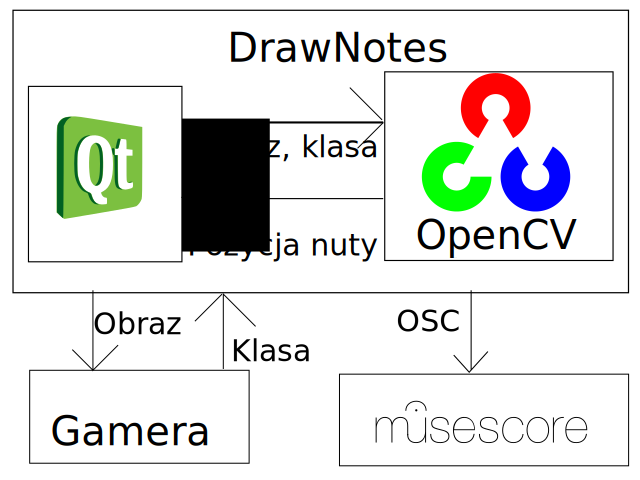
\includegraphics[scale=0.8,bb=0 0 512 384]{img/demo.pdf}
  \caption{Architektura programu DrawNotes}
  \label{demo}
\end{figure}

\newpage
\section{Diagram przypadków użycia}
Diagram przypadków użycia opisuje podstawowe czynności jakie może wykonać użytkownik z~pomocą programu DrawNotes.
\begin{figure}[H]
  \centering
  \includegraphics[scale=0.75,bb=0 0 505 735]{img/UC.png}
  \caption{Diagram przypadków użycia programu DrawNotes}
  \label{uc}
\end{figure}

\chapter{Implementacja programu}
\section{Proces rozpoznawania symboli}
Do realizacji programu DrawNotes użyto następujących pakietów oprogramowania Qt~\cite{Qt}, Gamera~\cite{Gamera} oraz OpenCV~\cite{OpenCV}.

Rozpoznanie nuty odbywa się z~wykorzystaniem projektu Gamera. Klasyfikacja odbywa się z~pomocą algorytmu k~najbliższych sąsiadów oraz następujących cech obrazu:

\begin{itemize}
  \item moments --- momenty obrazu. Ich definicję można znaleźć m.in. w~książce ,,Digital Image Processing''~\cite{Gonzalez:2006:DIP:1076432}.
  \item nholes --- oblicza dla każdego wiersza lub kolumny średnią liczbę białych przebiegów niedotykających brzegu. Z~tych liczb, zwracana jest średnia dla wierszy i~kolumn.
  \item nholes\_extended ---  dzieli obraz na cztery paski i~wtedy wykonuje analizę nholes na każdy z~pasków. Jest to wykonywane wertykalnie i~następnie horyzontalnie, co w~rezultacie daje osiem wartości cech.
  \item volume --- procent czarnych pikseli wewnątrz prostokątnej obwiedni obrazu.
  \item zernike\_moments --- oblicza wartości absolutne znormalizowanych momentów Zernike, które są niezmienne dla operacji skalowania, rotacji i~odbicia. Ich definicję można znaleźć m.in. w~książce ,,Image Analysis by Moments''~\cite{Pawlak}.
\end{itemize}

Powyższe opisy powstały głównie poprzez tłumaczenie opisów cech znajdujących się na stronie internetowej projektu Gamera~\cite{Gamera:features}.
Użyty został algorytm k~najbliższych sąsiadów, gdzie $k = 1$, ponieważ w~dokumentacji Gamera czytamy ,,During classification, you can choose two parameters: the parameter k~in the kNN classifier, and the set of features. The choice of k~depends on the minimum number of training samples you have for each class. [...] in most practical cases this boils down to k~= 1, unless you have an abundant amount of training data''~\cite{Gamera:tutorial}. Na wejściu algorytmu k-nn mamy: zbiór obiektów na podstawie, których przebiegać będzie klasyfikacja (dane treningowe), obiekt do sklasyfikowania, oraz parametr k. Na wyjściu otrzymujemy decyzję, do której klasy został zaklasyfikowany obiekt. Algorytm składa się z~dwóch kroków:

\begin{enumerate}
  \item Poszukaj obiektów najbliższych w~stosunku do obiektu klasyfikowanego na podstawie cech obiektów,
  \item Określ klasę obiektu klasyfikowanego na podstawie obiektów najbliższych.
\end{enumerate}

Dla każdego symbolu przygotowano zestaw jego 25 wzorcowych obrazów. Poniżej przykładowe symbole.

\begin{figure}[H]
  \centering
  \includegraphics[scale=0.2,bb=0 0 1637 656]{img/sample.png}
  \caption{Przykładowe ręcznie narysowane symbole nut}
  \label{symbols}
\end{figure}

Rozpoznanie wysokości nuty odbywa się trójetapowo:

\begin{enumerate}
  \item Obraz jest segmentowany na spójne części,
  \item W~przypadku całej nuty oraz półnuty następuje zamalowanie dziur z~wykorzystaniem: algorytmu Canny~\cite{OpenCV:canny} do znajdowania konturów obrazu; momentów Hu~\cite{OpenCV:moments} do obliczenia centrum dziury; algorytmu floodFill do zamalowania dziury~\cite{OpenCV:floodFill}. Następnie dla wszystkich nut z~wyjątkiem całej nuty następuje morfologiczne zamykanie w~celu usunięcia lasek nut~\cite{OpenCV:closing},
  \item Ostatnim krokiem jest wykonanie algorytmu fitEllipse~\cite{OpenCV:fitEllipse} na konturach zmodyfikowanego obrazu w~celu poznania współrzędnych środków główek nut.
\end{enumerate}

\newpage
\begin{figure}[H]
  \centering
  \includegraphics[scale=0.45,bb=0 0 688 1519]{img/graph.pdf}
  \caption{Diagram klas programu DrawNotes}
  \label{uml}
\end{figure}

\section{MuseScore}
Konieczna była implementacja obsługi następujących akcji wywoływanych za pomocą protokołu OSC:

\begin{itemize}
  \item next-chord, prev-chord --- przejdź do następnego, poprzedniego akordu,
  \item next-measure, prev-measure --- przejdź do następnego, poprzedniego taktu,
  \item backspace --- obsługa klawisza backspace --- cofanie zmian,
  \item pad-note-X --- wybierz czas trwania wprowadzanych nut (gdzie X przyjmuje wartości: 1, 2, 4, 8, 16, 32),
  \item add-pitch --- dodaj w~bieżącym miejscu nutę o~zadanej wysokości i~poprzednio określonym czasie trwania (patrz wyżej).
\end{itemize}

\section{Testy}
\subsection{Klasyfikacja}
Przygotowałem skrypt testowy, który działa następująco:

\begin{enumerate}
  \item Pobiera argumenty: testowany katalog z~plikami PNG, położenie skryptu klasyfikatora, położenie klasyfikatora XML,
  \item Dla każdego pliku w~testowanym katalogu klasyfikuje go i~sprawdza, czy przyznana klasa zgadza się z~klasą zadeklarowaną w~nazwie pliku (format "<klasa><nr>.png"),
  \item Wyświetla liczbę pozytywnie sklasyfikowanych obrazów.
\end{enumerate}

W~moich testach 100\% symboli testowych dużej rozdzielczości było rozpoznawanych. Natomiast symbole w~małej rozdzielczości były rozpoznawane w~około 80\% przypadków. Rozmiar danych testowych wynosił 5 dla każdego symbolu dużej rozdzielczości oraz 25 dla każdego symbolu małej rozdzielczości. Symbole testowe wyglądają podobnie do tych pokazanych wcześniej na rysunku \ref{symbols}.

\begin{figure}[H]
  \centering
  \includegraphics[scale=1.0,bb=0 0 605 340]{img/classify.png}
  \caption{Wynik eksperymentalnej klasyfikacji odręcznie narysowanych symboli testowych}
  \label{classify}
\end{figure}

W~teście źle wypada symbol ,,quarter'' czyli ćwierćnuta. Dzieje się tak prawdopodobnie ze względu na źle narysowane przykłady uczące, ze zbyt długą laską. Ponadto symbol ten był często błędnie rozpoznawany jako ,,eighth'', czyli ósemka.

\subsection{Próba czasowa}
Wykonałem próbę czasową dwóch sposobów wprowadzania notacji muzycznej --- wprowadzania za pomocą myszki oraz poprzez zbudowany program DrawNotes (pisanie ręczne). Do testu użyłem znanego utworu ,,Ave Maria'' J.S. Bacha \ref{avemaria}.

\begin{figure}[H]
  \centering
  \includegraphics[scale=0.5,bb=0 0 816 534]{img/AveMaria.png}
  \caption{Przepisywany utwór --- Ave Maria J.S. Bacha.}
  \label{avemaria}
\end{figure}
\begin{figure}[H]
  \centering
  \includegraphics[scale=0.95,bb=0 0 605 340]{img/time.png}
  \caption{Próba czasowa}
  \label{time}
\end{figure}
Z~rysunku \ref{time} można odczytać, że sposób wprowadzania notacji muzycznej przez pisanie ręczne jest około 2,5 raza wolniejszy (49 minut versus 126 minut).

\chapter{Podsumowanie i~wnioski}
Cel pracy został osiągnięty. W~szczególności udało się: dobrać i~zintegrować narzędzia do rozpoznawania i~cyfryzacji ręcznie sporządzonej notacji muzycznej w~postaci programu DrawNotes współpracującego z~MuseScore; przygotować zestawy danych treningowych (25 obrazów dla każdego symbolu) i~testowych (30 obrazów dla każdego symbolu: 25 małej rozdzielczości i~5 dużej rozdzielczości); przeprowadzić i~udokumentować testy (jakości klasyfikacji oraz szybkości przepisywania utworu); zbadać ankietowo znajomość narzędzi notacji muzycznej wśród użytkowników MuseScore i~LilyPond.

Podczas testów okazało się jednak, że dokładność rozpoznawania symboli w~małej rozdzielczości różni się od dokładności dla symboli z~dużym DPI (ang. dots per inch), co wpływa na szybkość interakcji, ze względu na błędy rozpoznawania symboli. Dla symboli w~małej rozdzielczości uzyskano dokładność rozpoznawania symboli wynoszącą około 80\%. Przeprowadzone eksperymenty pokazały, że praca edycyjna z~użyciem opracowanego narzędzia jest 2,5 raza wolniejsza niż tradycyjne wprowadzanie nut myszką. Z~tego względu ocena metody jest negatywna.

Osiągniętym celem dydaktycznym, który jest efektem ubocznym pracy nad programem było poznanie 
klasyfikatorów Gamera, pakietów oprogramowania OpenCV oraz Qt. Jako że poruszany problem jest dość rozległy~\cite{bainb2001}, zrealizowane oprogramowanie implementuje tylko podstawową funkcjonalność tj. wstawianie nut o~różnym czasie trwania na pięciolinii do programu MuseScore za pośrednictwem protokołu OSC. W~szczególności program nie rozpoznaje łączonych nut, akordów pisanych w~skróconej formie. Pomimo prostoty zrealizowanego oprogramowania pozwala ono na ocenę zaproponowanej metody wprowadzania notacji muzycznej. W~porównaniu do pisania nut na papierze część użytkowników może poczuć się zniechęconych do korzystania z~tego typu edytorów ze względu na wolne tempo tworzenia partytur. Rekompensatą za wolniejsze tempo pracy jest elektroniczny zapis partytury i~możliwość błyskawicznego jej powielenia i~eksportu do wielu popularnych formatów danych (pliki dźwiękowe, obrazy, PDF, MusicXML). Kluczem do zwiększenia tempa pracy z~elektroniczną partyturą może być dopracowanie mechanizmu rozpoznawania symboli tak, by analizował on wprowadzane dane na bieżąco. Tego typu rozwiązania mogłyby zostać wprowadzone w~ewentualnych kolejnych wersjach opracowanego programu.

{
  \backmatter
  \chapter{Bibliografia}
  \printbibliography[heading=none,sorting=title]
}
\listoffigures
\listoftables

\appendix
\chapter{Przewodnik użytkownika}
\section{Instalacja}
\subsection{MuseScore}
Należy zainstalować MuseScore z~repozytorium GitHub: \url{https://github.com/musescore/MuseScore}. Instrukcje kompilacji znajdują się na stronie: \url{http://musescore.org/en/developers-handbook}. Po uruchomieniu MuseScore należy włączyć w~nim serwer OSC (ścieżka Edit/Preferences/, zaznaczyć OSC remote control) i~zrestartować program.

\subsection{Gamera}
Należy postępować zgodnie z~instrukcjami zawartymi na stronie \url{http://gamera.informatik.hsnr.de/download/index.html}.

\subsection{DrawNotes}
Ściągnąć Qt ze strony \url{http://qt-project.org/downloads}. Otworzyć QtCreator i~wczytać projekt wskazując plik qt.pro z~katalogu projektu (Plik/Otwórz plik lub projekt). Zbudować projekt (kombinacja klawiszy CTRL+B) i~uruchomić (kombinacja klawiszy CTRL+R).

\section{Obsługa}
\subsection{MuseScore}
Aby wykorzystać możliwości przygotowanego programu należy włączyć tryb wprowadzania nut (klawisz N).

\subsection{Gamera}
Opublikowany klasyfikator w~pliku XML można edytować, dodając nowe symbole trenujące. Procedura dodawania symboli do klasyfikatora jest opisana na stronie \url{http://gamera.sourceforge.net/doc/html/training_tutorial.html}. Przygotowałem również zestaw skryptów pomocnych w~tworzeniu klasyfikatora.

\begin{itemize}
  \item convert.sh --- z~plików svg tworzy obrazy PNG o~DPI 1200,
  \item montage.sh --- z~zadanego katalogu wypełnionego plikami PNG tworzy jeden obraz PNG,
  \item montage-all.sh --- wykonuje skrypt montage.sh dla zadanych katalogów,
  \item resize.sh --- zmniejsza rozmiar pliku PNG do 10\%,
  \item resize-all.sh --- wykonuje skrypt resize.sh dla zadanych plików,
  \item setup\_wacom\_tablet.sh --- ustawia krzywą nacisku tabletu firmy Wacom na taką, by zawsze był rejestrowany maksymalny nacisk --- przydatne podczas rysowania symboli.
\end{itemize}

Struktura katalogów symboli trenujących przedstawia się następująco:

\begin{itemize}
  \item montaged --- połączone symbole trenujące,
  \item png --- obrazy treningowe,
        \begin{itemize}
          \item mouse --- narysowane myszką,
          \item svg --- wygenerowane z~svg,
          \item tablet --- narysowane tabletem,
        \end{itemize}
  \item resized --- przeskalowane połączone symbole trenujące,
  \item svg --- nuty w~SVG,
  \item templates --- puste pliki xcf --- wzorce,
  \item test --- pliki z~symbolami testowymi,
        \begin{itemize}
          \item big --- symbole w~dużej rozdzielczości,
          \item small --- symbole w~małej rozdzielczości.
        \end{itemize}
\end{itemize}

Zmontowany i~przeskalowany plik można jednym poleceniem załadować do programu gamera\_gui, a~następnie wystarczy zaznaczyć wszystkie posegmentowane symbole i~nadać im właściwą klasę.

\subsection{DrawNotes}
Na pięciolinii prezentowanej przez program można rysować symbole. Po pewnym czasie od przerwania rysowania symbole są analizowane i~następuje komunikacja przez protokół OSC z~serwerem OSC wbudowanym w~MuseScore uruchomionym na tym samym komputerze. Program rozpoznaje akordy jako symbole rysowane koło siebie. Niestety bieżąca wersja MuseScore nie udostępnia wprowadzania akordów przez OSC, dostępne jest tylko wprowadzanie pojedynczych nut.
W~zakładce File/Settings można zmienić następujące ustawienia programu:

\begin{itemize}
  \item Additional lines --- liczba dodatkowych linii powyżej i~poniżej pięciolinii,
  \item Pen point size --- rozmiar pióra do rysowania,
  \item Lines distance --- szerokość odstępu wertykalnego pomiędzy liniami pięciolinii,
  \item Delay to analysis --- liczba milisekund bezczynności, po której następuje analiza narysowanego symbolu,
  \item Message timeout --- liczba milisekund, w~których trakcie wyświetlane są komunikaty programu na pasku statusu,
  \item OSC port --- numer portu do komunikacji z~serwerem OSC.
\end{itemize}

\end{document}
